% Advanced Intelligent Systems table-of-contents item.
% The text is 55 words. The graphic reuses the system loop and adds no result.
\textbf{ToC text:} Planned camera pointing does not establish that a physical
observation occurred. ECR-Cover closes this gap by linking first-coverage
planning, acknowledged execution, stable measured pose, fresh-frame evidence,
and baseline-preserving event repair. Four-camera experiments show lower
first-observation latency without sacrificing complete-coverage time, while
every reported coverage step remains traceable to synchronized pose--frame
evidence.

\medskip
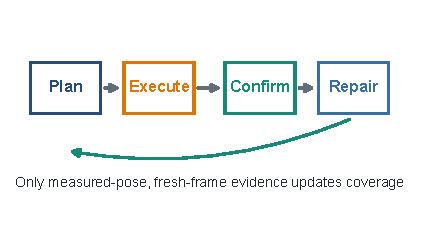
\includegraphics[width=85mm]{figures/toc_graphic.pdf}

